\chapter{If-Conversion \Author{C. Bruel}}\label{chap:if-conversion}
\inputprogress
\graphicspath{{img/}{if_conversion/img/}{part4/if_conversion/img/}}
	
\newcommand\cond{~?~}

%\setcounter{tocdepth}{3} 
%\tableofcontents

\section{Overview/Motivations}

We describe in this chapter an if-conversion algorithm in SSA. If-conversion is the process to optimize a control flow region into an equivalent region where branches have been removed. We start with a description of a full SSA model, taking as input a SSA region producing a SSA region using speculation. We then describe how this framework is extended to use predicated execution, using the $\psi$-SSA form presented in chapter ???. 

\subsection{Introduction}

A way to increase the instruction throughput is to increase the IPC (number of instructions per cycle), either by increasing pipeline depth, or by increasing the number of instructions that are executed simultaneously. This can be achieved by multiple issue processors. Either out-of-order superscalar execution models, using dynamic scheduling models and expensive hardware complexity or else in-order execution model in embedded processors because of lower hardware complexity, implying lower production and usage costs.

Instruction Level Parallelism (ILP) was demonstrated to be very effective on embedded processors, for example in the mathematical for evaluation of polynomial expressions \cite{Jeannerod:2010:TTI:1837210.1837212}, or to sustain performance in loop intensive computation required for multimedia applications \cite{FisherFaraboshiYoung}.

In order to exploit this ILP, those applications delegate to the compiler the responsibility to organize the parallel execution of the execution flow \cite{Rau:2003:IP:1074100.1074489}.

To permit the compiler to organize the parallelism explicitly, VLIW (Very Large Instruction World) or EPIC (Explicitly Parallel Architectures) make the parallelism visible into the ISA representation, relaying on the static scheduler to organize the compiler output so that multiple instructions can be issued for each cycle. 

Unfortunately, programs contain many sequences of instructions that cannot be parallelized, because of control or data dependencies. Different Instruction Level Parallelism techniques are implemented in the hardware, such as dynamic scheduling, branch prediction, or in the compiler, such as software pipeline, vectorization or loop optimizations. But still, despite those efforts, the execution flow is still disrupted by conditional branches, and many ALU cycles are wasted. 

Conditional branches introduce control dependencies between instructions. An instruction is control dependent on a preceding instruction if the first one determines the execution of the second one \cite{Kennedy:2001:OCM:502981}. They limit the scope of ILP optimizations, because they reduce the number of instructions that are not data dependent and thus can be executed in parallel. By reducing the average size of a basic block, they act as a bottleneck for exposing parallelism.

If-conversion is the process of transforming a control flow region containing several basic blocks into a single basic block of conditional instructions. Thus removing control branches from this region \cite{Schlansker97achievinghigh}. The conditional instructions are implemented on the target machine using the predication or speculation techniques described bellow.

Removing branches improves performance in several ways: by removing the mis-prediction penalty, the instruction fetch throughput is increased and the instruction cache miss penalty reduced. Enlarging the size of the basic blocks allows the static scheduler to schedule earlier long latency operations and to improve the ILP by merging multiple control paths into a single flow of execution. Many compiler optimizations are impacted by branches. Software Pipelining for example, cannot efficiently schedule loops with conditional branches \cite{Warter:1992:EMS:144953.145796}.

Consider the simple example \ref{fig:example1}, that represents the execution of an if-then-else statement on a 4-issue processor. Branches are highly biased (a branch is highly biased when it is known to be frequently taken or not), so the basic blocks can be reordered to favor the critical path. Even with this optimistic case, the schedule height is still 5 cycles (assuming that all instructions have a one cycle latency), with a maximal schedule height of 6 instructions. 

\begin{figure}
\footnotesize
  \subfloat[Control Flow] {
    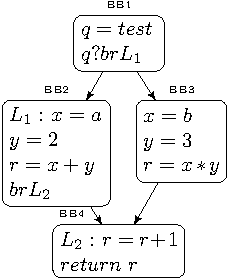
\includegraphics{specul}
    \label{fig:orig}}

  \subfloat[with basic block ordering] {
     \begin{tabular}[t]{lllll}
      & ALU1 & ALU2 & ALU3 & ALU 4 \\
\hline
      & $q = test$         &   -     &   -   & - \\
      & $q \cond br$ $L_1$ & -       & - & - \\
      & $x = 2$            & $y = 3$ & - & - \\
      & $r = x * y$ & - & - & - \\
$L_2$ & $r = r + 1$ & $return$ $r$  & - & - \\
$L_1$ & $x = a$ & $y = 2$ & - & - \\
      & $r = x + b$ & - & - & - \\
      & $br$ $L_2$ & - & - & - \\
     \end{tabular}}
\vspace{1cm}
  \subfloat[After if-conversion] {
     \begin{tabular}[t]{llll}
      ALU1 & ALU2 & ALU3 & ALU 4 \\
\hline
      $q = test$ & - & - & - \\
      $x_1 = 2$ & $y_1 = 3$ & $x_2 = a$ & $y_2 = 2$ \\
      $r_1 = x_1 * y_1$ & $r_2 = x_2 + y_2$ & - & - \\
      $r = q \cond r_1 : r_2$ & $return$ $r$  & - & - \\
       & & & \\     
       & & & \\     
       & & & \\     
       & & & \\     
     \end{tabular}}
\caption{Static schedule of a simple region on a 4 issue processor}
\label{fig:example1}
\end{figure}

After if-conversion the execution path is reduced to 4 cycles, regardless of the tests outcomes. 

From this introductory example, we can observe that the transformation implies:

\begin{itemize}
\item The merge of execution paths into a single execution path, implying a  better exploitation of available resources.  
\item The reduction of the schedule length, because instructions can be speculated before the branch.
\item That the ariables need to be renamed, 
\item The introduction of a \textit{merge} pseudo operation.
\item The production of new data dependency. If-conversion transforms control dependencies into data dependencies \cite{Allen:1983:CCD:567067.567085}. 
\end{itemize}

Considering that the merging point can be materialized into the original control flow by the $\phi$ pseudo operation and that the renaming is a basic property of SSA, the transformation from SSA to If-converted code seems straightforward.

\subsection{Architectural requirements}
The example illustrates also that the \textit{merge} pseudo operations needs to be mapped to a conditional form of execution on the target's architecture. Depending on the available support, the algorithm must be able to match the ISA, to provide support for conditional execution of instructions, or to conditionally commit the result of an instruction.
Basically, several kinds of support for predication can (co-)exist: predicated execution  or speculative execution by mean of conditional moves. A partial predication model is used to predicate only the subset of the ISA that are not easily speculable, usually memory operations.

Predication is an architectural feature that allows an instruction to be executed conditionally by means of a predicate.

\begin{figure}
\footnotesize
\begin{minipage}[t]{3cm}
\mbox{fully predicated} \\
$p \cond x = a + b $ \\
$\overline{p} \cond x = 0 $ \\
\end{minipage} 
\begin{minipage}[t]{3cm}
\mbox{select} \\
$t = a + b $ \\
$x= p \cond t : 0 $ \\
\end{minipage}
\begin{minipage}[t]{3cm}
\mbox{cmov} \\
$t = a + b $ \\
$x = 0 $ \\
$x = cmoveq$ $t$ \\
\end{minipage}
\caption{Conditional execution using different models}
\label{fig:pred}
\end{figure}

Speculation is a compiler technique that allows instructions that are control dependent to be executed unconditionally. The result can be committed only when the condition is known to be true. Examples of conditional moves are the $cmov$ (Pentium Pro) or the $select$ (Multiflow, ST231 VLIW) instructions.

Example \ref{fig:pred} shows a conditional execution using the different modes.

To be speculated, an instruction should not potentially create any other side effects, or hazards. For instance a memory load should not trap (cache misses can also be considered for performance). This of course prevents unconditional execution by means of speculation of memory access for which the address is valid only on the selected path. Because of those reasons memory operations are a major impediment to ILP. 

Since load are long latency operations, speculative load support is effective to fetch datas earlier in the instruction stream, reducing stalls. Modern architectures provide architectural supports to dismiss invalid address exceptions. Examples are the $ldw.d$ dismissible load operation of the $ST231$ processor or the $IA64 speculative loads$. Note that $IA64$ provides both speculative and predicate loads, so the former will be preferred by if-conversion. 

\begin{figure}
\begin{minipage}[t]{4cm}
\mbox{IA64 speculative load} \\
$t = ldw.s(addr) $ \\
$jump$ $l_1:$ \\
$check.s\:t$ \\
$x = t$ \\
\end{minipage}
\begin{minipage}[t]{4cm}
\mbox{Multiflow dismissible load} \\
$t = ldw.d(addr) $ \\
$x = select\: \cond t : x $ \\
\end{minipage}

\begin{minipage}[t]{4cm}
\mbox{base store hoisting} \\
$x=select\:p \cond addr : dummy $ \\
$stw (x, value) $ \\
\end{minipage}
\begin{minipage}[t]{4cm}
\mbox{index store hoisting} \\
$index=select\:p \cond i : j $ \\
$stw (x[index], value) $ \\
\end{minipage}
\label{fig:spec}
\caption{Example of speculated memory operations}
\end{figure}

Stores can be performed by speculating the address value, and forcing it to be a dummy valid address in the case of not taken path. Naturally store hoisting can only be done if there is no aliasing conflict between different memory operations merged into a single execution path.

\section{Classical If-Conversion process}

Established if-conversion processes addresses the problem in the following order. First allocates boolean variables to the basic blocks, on an identified sub-region, then perform predicate initialization placement and then restructure the CFG sub-region into the final if-converted region. 
As an starting example we describe briefly the RK algorithm proposed by Park and Schlansker \cite{Schlansker-predicated} on the nested tests from figure In \ref{fig:nested1}. 
The RK algorithm starts to compute the Control Dependence Graph \cite{Ferrante:1987:PDG:24039.24041}. It is necessary to map the basic blocks to guard conditions, and the guards and the set of basic blocks that need to set them. The algorithm creates a new guard, eventually initialized to false, for each condition. \ref{fig:nested1_rk.pdf} shows the sub-region with new conditions initialized, and \ref{fig:RK} the RK mappings.

\begin{figure}
\centering
  \subfloat[Nested test] {
    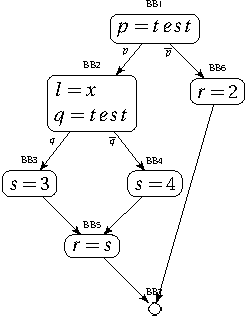
\includegraphics[scale=0.8]{nested1}
    \label{fig:nested1}}
  \subfloat[Predicate Assignments] {
    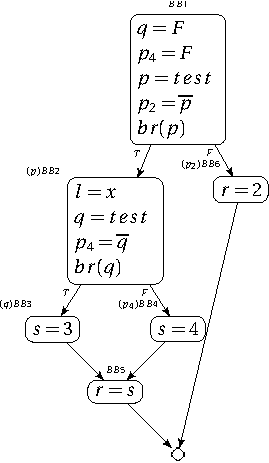
\includegraphics[scale=0.8]{nested1_rk}
    \label{fig:nested2}}
  \subfloat[After Instruction layout] {
    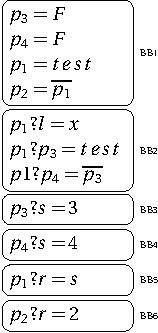
\includegraphics[scale=0.8]{nested1_rk2}
    \label{fig:nested}}
\caption{Classical support for partial predication}
\label{fig:trad_part_pred}
\end{figure}

\begin{figure}
\footnotesize
  \subfloat[R mapping] {
     \begin{tabular}[t]{|l|cccccc|}
\hline
      Basic Block & BB1 & BB2 & BB3 & BB4 & BB5 & BB6  \\
\hline
      Guard       &  T  &  p   & q  & p4  &  p  &  p2 \\
\hline
     \end{tabular}}
  \subfloat[K mapping] {
     \begin{tabular}[t]{|l|cccc|}
\hline
      Guard          & p & q & p4  & p2  \\
\hline
      Basic Block    & 1 & 2,-0 & -2,-0 & -1 \\
\hline
     \end{tabular}}
\caption{Output from RK algorithm}
\label{fig:RK}
\end{figure}

The process finishes by emitting the conditioned instructions, and removes the branches. \ref{fig:nested2_rk2}. 

There are several problems with this approach. First, it strongly assumes that all instructions can be predicated, in particular predicate setting operations (test) need to be conditioned. Without predicated support for comparison instruction, a merge must be done between the condition setting. For instance in the given example the initialization sequence $p_1 ? p_3=test$ needs to be rewritten as $t=test; p_1=p_3 \& t$. Speculative based approach, necessary to handle efficiently partially predicated architectures are then penalized by this approach, since a rewritten pass is needed to convert a conditional instruction into a temporary register and a conditional move.
Another pitfall, the algorithm works a a pre-selected control flow subregion. One of the challenge of all if-conversion frameworks is to be able to predict that the conversion will be beneficial before effectively doing it. If the  the number of computed guards exceed the number of predicate registers, then a new region has to be re-considered and the process restarted. Even with full predication support, speculative execution can be beneficial. Traditional algorithm tend to predicate all the instructions defined by a basic block, without considering their use. For instance in $BB2$ the instruction $l=x$ doesn't have any use other than the done defined by its predicate. Finally, those framework required intensive computing resources to compute the Control Dependence Graph, Register Renaming, a Def-Use chains or post-phase Predicate Reduction processing.

We propose in the remaining of the chapter an application of SSA to efficiently deal with those problems

\section{SSA If-Conversion}

SSA provides an efficient intermediate representation in which false data dependencies have been removed, removing the need for register renaming when merging two definitions into one. Each assignment target (def) is assigned a unique register name. Registers are re-materialized at join nodes using $\phi$ operations. A procedure is in minimal SSA form if the number of $\phi$ instructions at join nodes is as small as possible. In relation to if-conversion, The SSA representation ensures that a variable is assigned only once, and their merging point is exposed as $\phi$ operations. SSA alleviates the need for renaming and only the definitions used in a $\phi$ need to be predicated. 

Consider the equivalent SSA representation of the example \ref{fig:nested1}.

\begin{figure}
\centering
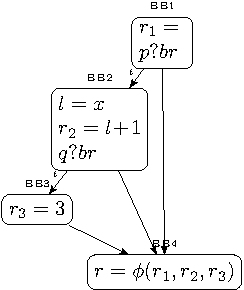
\includegraphics[scale=0.8]{nested4}
\caption{Nested test in SSA}
\label{fig:nest_ssa}
\end{figure}

Note that basically, since a $\phi$ expresses the merging point of $n$ definitions from $n$ predecessors. Thanks to SSA the definition point is immediately available, since it corresponds to the path by which the $\phi$ operand is reached. By construct, the definition of a $\phi$'s use is control dependent from the first condition that dominates it. For example, $s \phi$'s use in $BB3$ is control dependent of $BB2$. Locally, SSA information replace the need for a control dependence graph, which is an engineering advantage. Since $\phi$ functions are optimally placed thanks to the iterated dominance frontier criterion, we know that the predicate definition will be optimal, so a minimal set of condition is needed.

A very big difference in nature is in the way the merging of conditional is realized using data dependencies instead of predicate selection. In SSA the condition merge assignment is not realized thru merging of predicates, but using two successive conditional moves operations.

This algorithm takes as input a structured region in pure SSA form and produces a pure SSA using conditional move instructions to realize join points. One benefit of this approach is that all SSA properties are maintained, and scalar optimizations, such as constant propagation, can be executed without predicate awareness. Without SSA speculative if-conversion, implementation of a predicated intermediate representation is very complex, because optimization and def-use chains must deal with partial definitions.

\subsection{SSA operations on basic blocks}

\begin{figure}[h]
\centering
  \subfloat[phi removal] {
  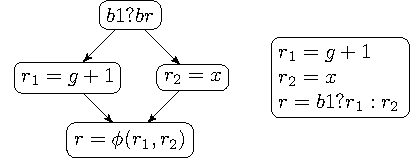
\includegraphics[scale=0.8]{phi_removal}
  \label{fig:phi_rem}}
  \subfloat[phi reduction] {
  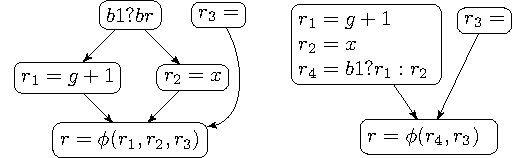
\includegraphics[scale=0.8]{phi_reduction}
  \label{fig:phi_red}}

  \subfloat[phi augmentation] {
  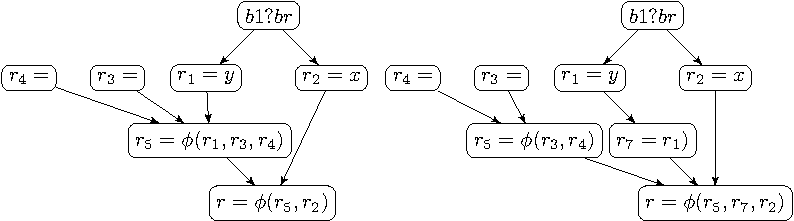
\includegraphics[scale=0.8]{phi_augmentation}
  \label{fig:phi_aug}}
\caption{SSA transformations}
\label{fig: phi_operations}
\end{figure}

The basic control flow structure for the transformation is based on hammocks graphs. A hammock is a single-entry single-exit control flow region $H$ with a distinguished entry node in $H$ and a distinguished exit node not in $H$. \cite{Ferrante:1987:PDG:24039.24041} and was demonstrated to be efficient for parallelization and global code optimization \cite{Zhang:2004:UHG:977250.977393}. Is is also very powerful for predication because the describe a well defined scope and the number of conditional variables are minimized.

We restrict for now the transformation to the speculative and conditional move model. We use the $select$ like notation $r=c?:r_1:r_2$, to represent the speculative execution of instruction defining $r_1$ and $r_2$. $r$ takes the value of $r_1$ if $c$ is True, else $r_2$. We will study how to generate code for predicated instruction in the next section.

Consider a conditional branch depending on a predicate $p$ and a region starting at $BBhead$. Let $BBp$ be the set of single exit basic blocks $(BBi,\dots,BB_n)$ that are on the taken path if $p$ is true and $BBq$ be the set of single exit basic blocks $(BBj,\dots,BB_m)$ that are executed if $p$ is false. The merge point of the if-converted region is at $BBjoin$. We distinguish 4 types of basic SSA transformations:

\subsubsection{$\phi$ removal} (figure \ref{fig:phi_rem})
The join node of the considered region has two predecessors and $\phi$ instructions are of the form $r=\phi(r_1,r_2)$. After speculation of the definitions of $r_1$ and $r_2$ the instruction can be rewritten as $r=p?r_1:r_2$.
Once $BBp$ and $BBq$ have been promoted into $BBhead$, $BBjoin$ has for only predecessor $BBhead$ so it is not in its dominance frontier. The $\phi$ can then be discarded.

\subsubsection{$\phi$ reduction} (figure \ref{fig:phi_red})
 The join node of the considered region has $n$ predecessors that have $\phi$ instructions of the form $r=\phi(r_1,r_i,r_j,\dots,r_n)$. After merging, the $\phi$s are rewritten $t=p?r_i,?r_j$ and a new $\phi\:r=\phi(r_1,t,\dots,r_{n-1})$ is created with one operand less. The merging instruction is inserted after the speculated $r_i$ and $r_j$ definitions into $BBhead$.
$BBjoin$ is still in the dominance frontier of $BBhead$, A $\phi$ must be redefined with the new definitions. The two corresponding $\phi$ edges from $BBq$ and $BBp$ can be replaced by the $BBhead$ edge.
The join block $E$ has $n$ predecessors with $n > 2$, and $n$ blocks in its dominance frontier if it contains $\phi$s.

\subsubsection{$\phi$ augmentation} (figure \ref{fig:phi_aug})
The objective is to remove incoming edges into the region, so the code is restructured during the if-conversion process to form a hammock. Consider a join node with $n$ predecessors among which $p$ is duplicated into $q$.  The join node of the considered region have $\phi$ instructions of the form $r=\phi(r_1,p,r_i,r_j,\dots,r_{n-1})$. The instruction is rewritten $t=select(p,r_i,r_j)$ and \mbox{$r=\phi(r_1,t,q,\dots,r_n)$}. 
The duplicated blocks are new dominators of $BBjoin$ that define new $defs$. These blocks are now in the dominance frontier of $BBjoin$. SSA is maintained with new $\phi$ upgraded with the new reaching points.

Since data flow dependencies are broken, new opportunities for propagation or scalar optimization arise. Here the local $t$ appears temporary, since $r2$ can be propagated into the $\phi$.

A difficulty is that in a Hammock region, eg no side entries, the control dependency $\phi$ operands's definition $BBp$ is easily deduced from its first dominator. However the $BBp$ is not necessary a direct successor of the $BBhead$, therefore, knowing that we are control dependent is not enough. We also need to know if the dependencies is on the false condition or the true condition, This is easily solved by walking back the chain of basic blocks until the edge coming from $BBhead$ is found.

\subsection{SSA representation of conditional instructions}

One problem of the described SSA-speculative framework is that it doesn't fit very well with a predicated model of conditional execution. Since $\phi$ are transformed to realize joint points into conditional moves, we should backtrack to relink the conditional moves into predicated instructions. This process of transforming speculation into predication is not convenient for many reasons:
- Predication introduces a renaming problem: Since a same register name can have 2 different assignments (under different predicates), this breaks SSA rules. The solution is to re-use the framework to realize join points into an extended SSA representation:

In \cite{Stoutchinin:2001:ESS:563998.564022} $\psi$-SSA was described as a way to express a predicated form of SSA extension. Such representation is usually built from already predicated code, non SSA, originating from inlined assembly, peepholes, intrinsics functions or local transformations of control flow idioms. 

$\psi$-SSA expose the edge dependency from the basic block into which the definition of the $\phi$ argument is defined in the original CFG by a new data dependency. This dependency needs to be materialized into a $select$ or $\psi$ operation. Note that the $select$ operation is a real instruction that don't need to be replaced by the out-of-ssa process. If the target architecture doesn't provide such instruction to switch between speculated instruction, it can be emulated using two conditional moves. One advantage to generate $select$ instruction at this stage is that the program stays in full SSA form and make all the data dependencies explicit, and can be feed to all SSA optimizers. 

\begin{figure}
\begin{minipage}[t]{3.5cm}
\mbox{SSA:} \\
$ if (p) $ \\
$   x_1 = a+b $ \\
$ else $ \\
$   x_2 = 0 $ \\
$ x = \phi (x_1, x_2) $ \\
\end{minipage}
\begin{minipage}[t]{3.5cm}
\mbox{SSA-speculative form:} \\
$x_1 = a + b $ \\
$x_2 = 0 $ \\
$x = p \cond  x_1 : x_2$ \\
\end{minipage}
\begin{minipage}[t]{3.5cm}
\mbox{$\psi$-SSA form:} \\
$x_1 = a + b $ \\
$x_2 = 0 $\\
$x = \psi (p \cond x_1, \overline{p} x_2) $ \\
\end{minipage}
\end{figure}

Note that unlike $\phi$ arguments that are executed simultaneously (they don't depend each other), $\psi$ arguments are executed sequentially and ordered from their definition predicate set. This property is necessary because of the new data dependencies introduced into the the straight line of predicated code stream.

The basic idea behind the SSA transformations is to replace $\phi$ operations by predicated instructions merging into a $\psi$ or speculated instructions merging into a $select$ equivalent instruction, while maintaining the SSA properties.

\subsection{SSA promotion}

To know the values that need to be conditionally defined, we only need to look at the defining instructions of the $\phi$ instructions. By elimination, all temporaries that do not have a join point into the considered region and that don't have a side effect are unconditionally speculated during the SSA transformations processes. Instructions with a side effect will need to be guarded. This is a considerable advantage over traditional if-conversion algorithms that marks all instructions in a conditional basic block as dependent on the predicate. By removing this predicate dependency, which is a data dependency, the instruction can be moved before the predicate assignment.

Our algorithm is applied iteratively on a control flow in SSA form until no more reductions are possible. The quality of the SSA taken as input does not affect the correctness of the algorithm: if the control flow is in pruned SSA, i.e two paths $x->+z$ and $y->+z$ converge at node z, then a $\phi$ node is inserted at z only if z is alive in or after z. if which case x and y are promoted and no $select$ operation is generated. If the SSA is minimal, a $select$ instruction would be generated and removed by dead code. Inserting dead code from minimal SSA only introduces noise in the local scheduling heuristics because of the false data dependencies.

\subsubsection{Partial redefinition}

A $\psi$ operation exposes new data dependencies, by expressing the merge of two definitions. Note that the order of the partial definition is important, so a definition partially redefines the preceding ones. We use this property to speculate the first definitions, so it becomes speculated instead of disjoint. This local optimization allows the removal of apredicate dependency but also creates a new partial dependency (predicates are not disjoint). 

\begin{figure}
\footnotesize
\begin{minipage}[t]{4cm}
\mbox{disjoint predicates} \\
$ p = test $ \\
$ p \cond x_1 = a + b $ \\
$ \overline{p} \cond x_2 = c $ \\
(1) $ x = \psi(p \cond x_1, \overline{p} \cond x_2) $ \\
\end{minipage}
\begin{minipage}[t]{4cm}
\mbox{optimized order predicates} \\
$ x_1 = a + b $ \\
$ p = test $ \\
$ \overline{p} \cond x_2 = c $ \\
$ x = \psi(T \cond x_1, \overline{p} \cond x_2) $ \\
\end{minipage}
\end{figure}

$T$ represents the $True$ predicate. This optimization is useful to save one predicate register and to remove a data dependency between a predicate definition in its use. 
The $\psi$ definition is defined on the $T$ predicate set, therefore it is speculable, as shown here:

\subsubsection{$\psi$ speculation properties}

Since $\psi$ operations are part of the intermediate representation, they can be considered for inclusion in a candidate region for if-conversion. Conditional operations defined are thus in turn speculated or conditioned. We define here promotion rules for $\psi$ operands, whereas the instructions defining the $\psi$ operands will be speculated, and the condition realized by the use of the $\psi$ definition.

Consider the instructions \ref{nest_psi} containing a subregion already processed. The $\psi$ operation can be safely speculated if all the instructions defining its operands can be speculated. So 1) they don't produce hazardous execution and they don't produce any side effects, 3) there exist a conditional move instruction to merge the results. Then the block can be executed regardless of the value of $c$. The use of the $\psi$ result is also unconditionally executed, and the condition realized in the $\phi$ transformation.

\subsubsection{$\psi$ predication properties}

If the instructions are not speculable, they must be predicated:
In \ref{fig:nested_psi_predicated}, the $c$ condition merges with all conditions under which the $\psi$ operands are defined. Here a new predicate $p_1$ is created to hold the predicate definition for the instructions defined under $c$. 

Note that conceptually, the speculative $\psi$ execution allows a predicate definition domain larger that the original one, which the predicative transformation exactly matches the initial definition domain, at the expense of more data dependencies and predicate computation.

We can see with this example that the decision to speculate or predicate can be done at the level of each joining definition, allowing a mix of them in the final program. The advantage to speculation over predication is a reduced dependency length. The disadvantage of speculation is that it increases register pressure until the merge point, and puts long latency operations on the critical path.
 
\begin{figure}
\footnotesize
\begin{minipage}[t]{3.5cm}
\mbox{nested if} \\
$ if (c) $ \\
$ \{ $ \\
\hspace*{2mm}$ x_1 = a + b $ \\
\hspace*{2mm}$ \overline{p} \cond x_2 = c $ \\
\hspace*{2mm}$ x = \psi(T \cond x_1, \overline{p} \cond x_2) $ \\
\hspace*{2mm}$ d_1 = use (x) $ \\
$ \} $ \\
$ else $ \\
\hspace*{2mm}$ d_2 = 3 $ \\
$ d = \phi(d_1,d_2) $ \\
\label{nested_psi}
\end{minipage}
\begin{minipage}[t]{3.5cm}
\mbox{speculated nested if} \\
$ x_1 = a + b $ \\
$ \overline{p} \cond x_2 = c $ \\
$ x = \psi(T \cond x_1, \overline{p} \cond x_2) $ \\
$ d_1 = use (x) $ \\
$ \overline{c} \cond d_2 = 3 $ \\
$ d = \psi(T \cond d_1, \overline{c} \cond d_2) $ \\
\label{nested_psi_speculated}
\end{minipage}
\begin{minipage}[t]{3.5cm}
\mbox{predicated nested if} \\
$ p_1 = \overline{p} \& {c} $ \\
$ c \cond x_1 = a + b $ \\
$ p_1 \cond x_2 = c $ \\
$ x = \psi(c \cond x_1, p_1 \cond x_2) $ \\
$ d_1 = use (x) $ \\
$ \overline{c} \cond d_2 = 3 $ \\
$ d = \psi(T \cond d_1, \overline{c} \cond d_2) $ \\
\label{nested_psi_predicated}
\end{minipage}
\caption{Inner region $\psi$}
\end{figure}

\subsubsection{Predicate merging}

During the region formation, subregions containing a block that is reached from two conditions can be optimized by merging predicates. A new predicate is computed using a logical operation on both basic blocks' predicates after a normalization pass. Simple logical operations are usually caught as a peephole or during the instruction selection mechanism, but making it part of the if-conversion process allows it to handle more complex regions because our predicate merging algorithm is not limited to basic blocks that only define predicates, making instructions depending on predicates merge part of the generic SSA speculation framework. However, this transformation is very sensitive to biased branches since each conditional operation now depends on two predicates instead of one that cannot be scheduled together because of the computation of the logical operation making it more difficult to compensate for the branch removal. In order to avoid long sequences data dependencies and break schedule, we exclude from this promotion predicates that depend on long latency operations.
Because of new data dependencies introduced by the new computed predicate the performance contribution of this transformation mainly comes from the branch removal (two conditional branches and two direct branches are removed from a if-converted region whose predicates have been merged) rather than local ILP. Predicate promotion and merge is more effective in loop nest regions where more optimizations may extract ILP from it, for example modulo scheduling can extract ILP from such if-converted bodies by overlapping different iterations. 

We allow two successive conditional blocks sharing one immediate post-dominator to be merged with logical operations after a normalization transformation. The normalization transformation ensures that conditional blocks sharing a common target can be merged by defining a wired $or$, or a wired $and$ share the same branch characteristics using branch reordering, test inversion or $de-morgan$ transformations.

\begin{figure}
  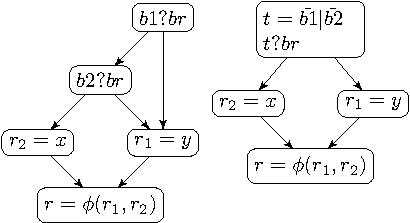
\includegraphics[scale=0.8]{phi_merge}
  \label{fig:phi_merge}
\caption{Predicate merging}
\end{figure}

\subsubsection{Block duplication}

Block duplication is used to remove side edges and to remove the constraints on control dependencies in order to enable the algorithm to find a set of basic blocks to if-convert. Unless applied carefully, block duplication could be the cause of code bloating without performance improvement. However experience has shown that when applied carefully it can be the source of very efficient if-conversion. 
Consider for example in the figure \ref{fig:bbdup}. Since we are if-converting from the inner most regions, the algorithm first considers the region {BB3,BB4,BB5,BB6,BB7}, and discards the edge coming from BB2 by duplicating BB6 into BB8. The $\phi$ becomes a move in the duplicated block with a renamed definition. The new $\phi$ operands are updated from the new edge. Note that in the implementation the block does not need to be created since it will be next promoted into BB3. We have two nested hammocks and the process can iterate. The dependency that we removed in the control flow is now expressed as a data dependency between the two $select$ instructions.

The algorithm to perform SSA block duplication is decomposed into three steps: 
\begin{itemize}
\item Extract the $\phi$s 's def to be conditioned from the duplicated block creating a $move$ instruction and a new reduced $\phi$ (or two $move$ instructions if the duplicated block had only two incoming edges).
\item Then the $\phi$s in the tail basic block are augmented with the new def created by the new repair instruction. If the $\phi$ was live-out after the tail block a move must be inserted to avoid propagating renaming outside of the region considered. 
\item The last step consists of renaming the new definitions to keep the region in SSA form.
\end{itemize}

\begin{figure}[h]
\centering
  \subfloat[Original] {
    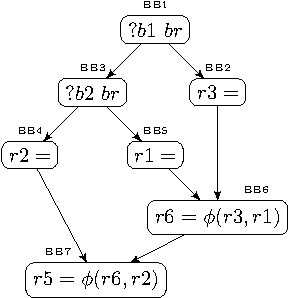
\includegraphics[scale=0.75]{side1}
    \label{fig:side1}}
  \subfloat[After duplication] {
    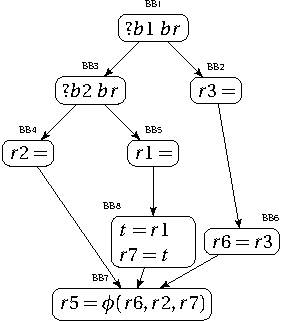
\includegraphics[scale=0.75]{side2}
    \label{fig:side2}}
  \subfloat[sub-region 1] {
    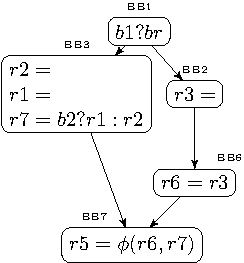
\includegraphics[scale=0.75]{side3}
    \label{fig:side3}}
  \subfloat[sub-region 2] {
    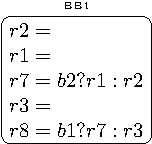
\includegraphics[scale=0.75]{side4}
    \label{fig:side4}}
\caption{Side entry removal using block duplication}
\label{fig:bbdup}
\end{figure}

\section{Hyperblock formation in SSA}

Unfortunately, critical regions are rarely composed of simple hammocks or one level nested ifs. At the same time, processors have limited resources. the number of registers will determine the acceptable level of data dependencies to minimize register pressure, the number of predicate registers will determine the depth of the if-conversion so that the number of conditions doesn't exceed the number of available predicates. 

The region must be just large enough to swell the scope of scheduling, without over-commiting the machine resources. On the contrary, although if-conversion removes branches, It also adds some overhead (new instructions to merge predicates, register pressure for speculative conditional, heigher dependence height because of the presence of new data dependencies on the predicates). The newly formed basic block should not have a higher schedule estimation than the one that would have been taken if the code was not if-converted.

For this reason, existing approaches to if-conversion are either limited to a single conditional branch using peepholes-style pattern matching, intrinsic functions (conditional code is inlined by the compiler in the internal representation), or scoping larger but restricted regions such as loops hyperblocks. Such approaches require that the region is isolated from the rest of the control flow, and it requires a complicated estimation of the future if-converted region.

A hyperblock \cite{Mahlke:1992:ECS:144965.144998} is a region of code with a single entry and possible, multiple exits where inner branches have been removed by if-conversion.
Hyperblock are the basis to enlarge the scope for scheduling in two ways: First, since basick blocks swell as the scope of predicated region grows, static scheduling can now be unconstrained, second, instructions can freely be speculated without the need for compensation code. Conditional code to exit the hyperblock does not impact the execution flow, using a proper code basic block reordering to favor fall thru execution.
Tail duplication is used to exclude from the Hyperblock basic blocks that can't be if-converted, either because the contain hazardous instructions, or because of heuristic decisions.

Generally, hyperblocks are created in the following steps:
\begin{itemize}
\item Create a trace and block selection. A trace is a sequence of basic blocks that can be scheduled together. 
\item Remove side entries with tail duplication, This step removes scheduling constraints imposed by side entries, or allow regions to be if-converted despite hazards.
\item Perform if-conversion.
\end{itemize}

We describe here how Hyperblocks are build using this SSA framework, and how they are inherently part of the if-conversion process.

\subsection{SSA Iterative if-conversion}

The region to if-convert must be carefully selected. Because of resource consumption issues, merging different paths together can over commit the architectural ability to execute in parallel the multiple instructions: The data dependences and registers renaming, introduce new register constraints. Moving operations earlier in the instruction stream increases live-ranges. 
Another pitfall is to increase the critical path by merging long latency operation from a less frequently executed path, thus moving to the critical paths more instructions than the parallelism can absorb.
Finally, for each basic block considered into the region, a predicate must be computed and assigned to the corresponding instructions. Those predicate computations introduce new instructions and new data dependencies.

More classical if-conversion algorithms cover the region-selecton and if-conversion separately, so the region is isolated first and then the work is left to the if-conversion algorithm. All those steps make the if-conversion process a complex optimization, forcing designers to be extremely conservative, as the objective functions must contain variables not known at the start of the transformation. (such as the complexity of the predicate equations) since moving multiple control paths together can easily exceed processors resources (leading to excessive register pressure) or move infrequently used expensive instruction (memory loads) into the critical path. 

In contrast, the SSA iterative based if-conversion  brings together region selection and region transformation, The algorithm is to walk the control flow iteratively 

The algorithm is straightforward. It iterates a structured directed control flow in postorder traversal the list of candidate conditional blocks of the control flow. Postorder traversal garantees that each inner region will be processed before the regions of larger scopes. No sub-region needs to be selected, because the decision to if-convert will be retaken incrementally which each nested gets if-converted and the Hyperblock grows. When the region cannot grow anymore because of resources, or because a basic block cannot be if-converted, then another region is considered.

The bigger adantage on an incremental optimisation of the control flow is that since nested regions are already predicated when evaluating the if-conversion of a branch, all side effects introduced by the if-conversion, such as new predicate merging instructions, new conditional moves merging flow or new data dependencies will be taken into account. Furtheremore, the predicate assignment is not needed, since new predicates are mechanically inserted when merging inner regions containing conditional code.

Since the algorithm processes the control flow in postorder traveral, the dominator tree does not change, and it's possible to maintain the SSA locally to the inner region. By recurrence the if-converted region can be in turn optimized out if it's head belongs to the dominance frontier of an outer region.

We have proposed a few transformations to convert control flow complex regions into nested Hammocks, such as Basic Block duplication and Predicate merging. The prevalent idea is that the inner region once predicated will be viewed as a single basic region by the outer scopes.

Consider for example the control flow transformations for the $wc$ program (figure \ref{fig:wc1}). Exit nodes is BB7. Nodes BB7 and BB3 contains 

 The postorder list of the basic nested regions is {BB11, BB17, BB16, BB14, BB10, BB9, BB6, BB2}. The head of nested hammocks is represented by circle nodes. The nodes BB3 and BB7 contains calls, so they need to be excluded from the if-conversion.
The first hammock region starting at BB11 to BB2 contains BB12, that is promoted and BB2 becomes the single successor of BB11. 
For the region starting at BB17, BB19 cannot yet be promoted because of the side entry, so it is duplicated into BB15, that has now BB2 as successor.
BB16 is the start of a region containing BB17 and BB19. The former can be merged from the 2 conditions coming from BB16 and BB17. BB17 can be promoted into BB16 under BB16's conditions and BB19 under BB16 and BB17 conditions. Note that at this stage BB16's successors are BB19 and BB2.
BB14 is the head of the newly created region where BB15, BB16 and BB17 can be promoted. From BB9 a merging predicate is computed with the one in BB10. Instructions in BB14 are conditionalized on this new predicate and BB10 promoted, forming a new hammock at BB9 with BB14 and BB11 that can be promoted. The last candidate, BB2 is the start of a region that cannot be promoted, because of the call in BB3.
The region is now if-converted, leaving a single back-edge, removing 7 branches inside the body loop. At this stage, a local decision can be made to decide if tail-call must be performed to form an hyperblock containing only BB2,BB5,BB6 and BB9, excluding BB3. 

\begin{figure}
  \subfloat[Before if-conversion] {
    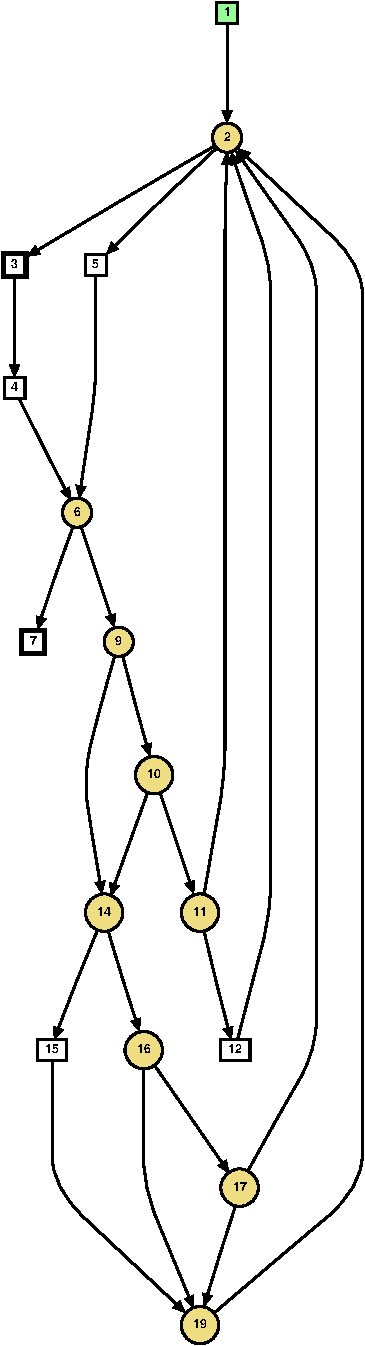
\includegraphics[scale=0.6]{graph1}
    \label{fig:wc1}}
  \subfloat[After if-conversion] {
    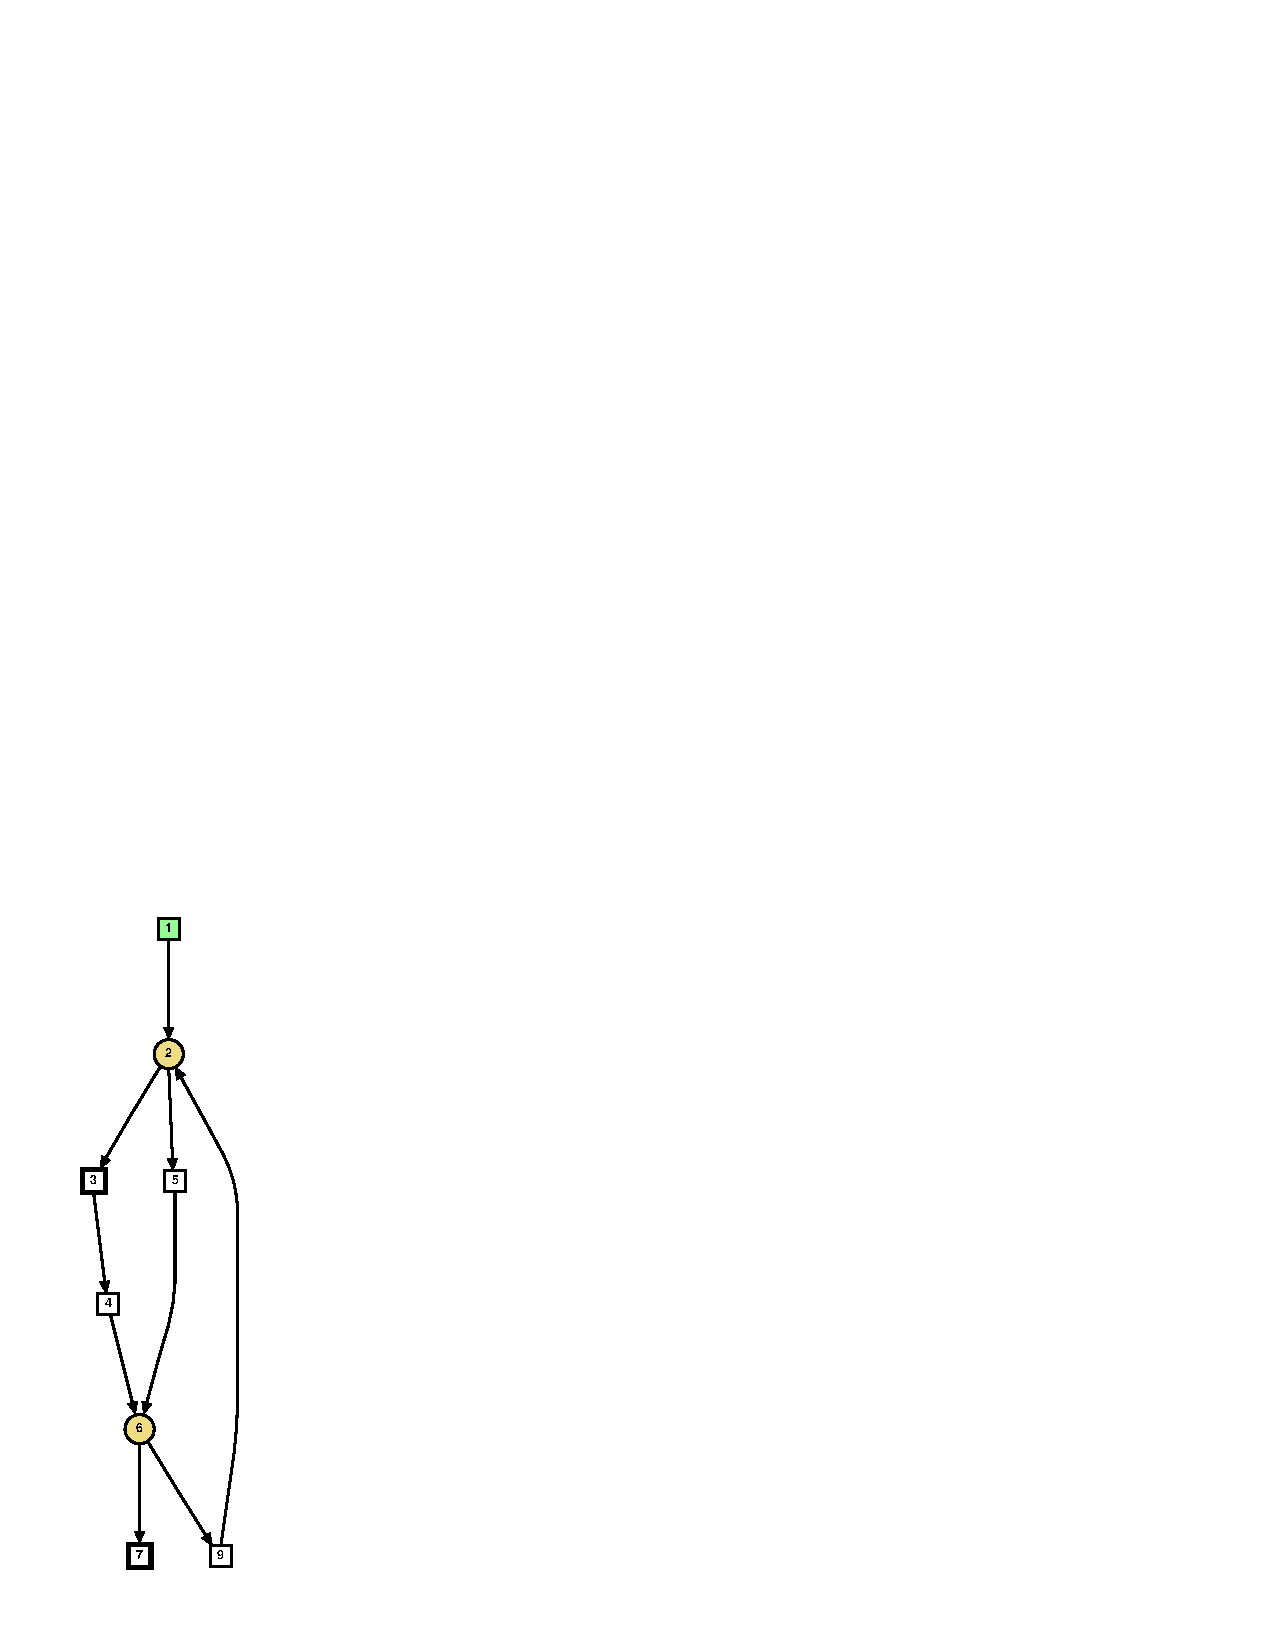
\includegraphics[scale=0.6]{graph7}
    \label{fig:wc2}}
\label{fig:wc example}
\end{figure}

\subsection{Tail Duplication}

Consider the example of Hyerblock formation \ref{fig:hyper1}. This loop contains two branches, and so if-converting it would be profitable. However, block selection has excluded BB2. and has integrated BB5, because heuristics have determined that the schedule of BB5 inside BB4 would be beneficial. The hyperblock contains {BB1, BB3, BB4, BB5, BB6}. Since BB4 has a side entry, it must be removed by tail duplication. \ref{fig:hyper2} shows the  control flow after block duplication. Notice that a new node, BB7 has been added after the tail duplication by a process called branch coalescing. Finally \ref{fig:hyper3} shows the code once if-converted.

\begin{figure}[h]
  \subfloat[loop] {
    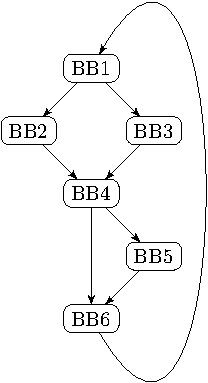
\includegraphics[scale=0.7]{hyper1}
    \label{fig:hyper1}}
  \subfloat[standard tail-duplication] {
    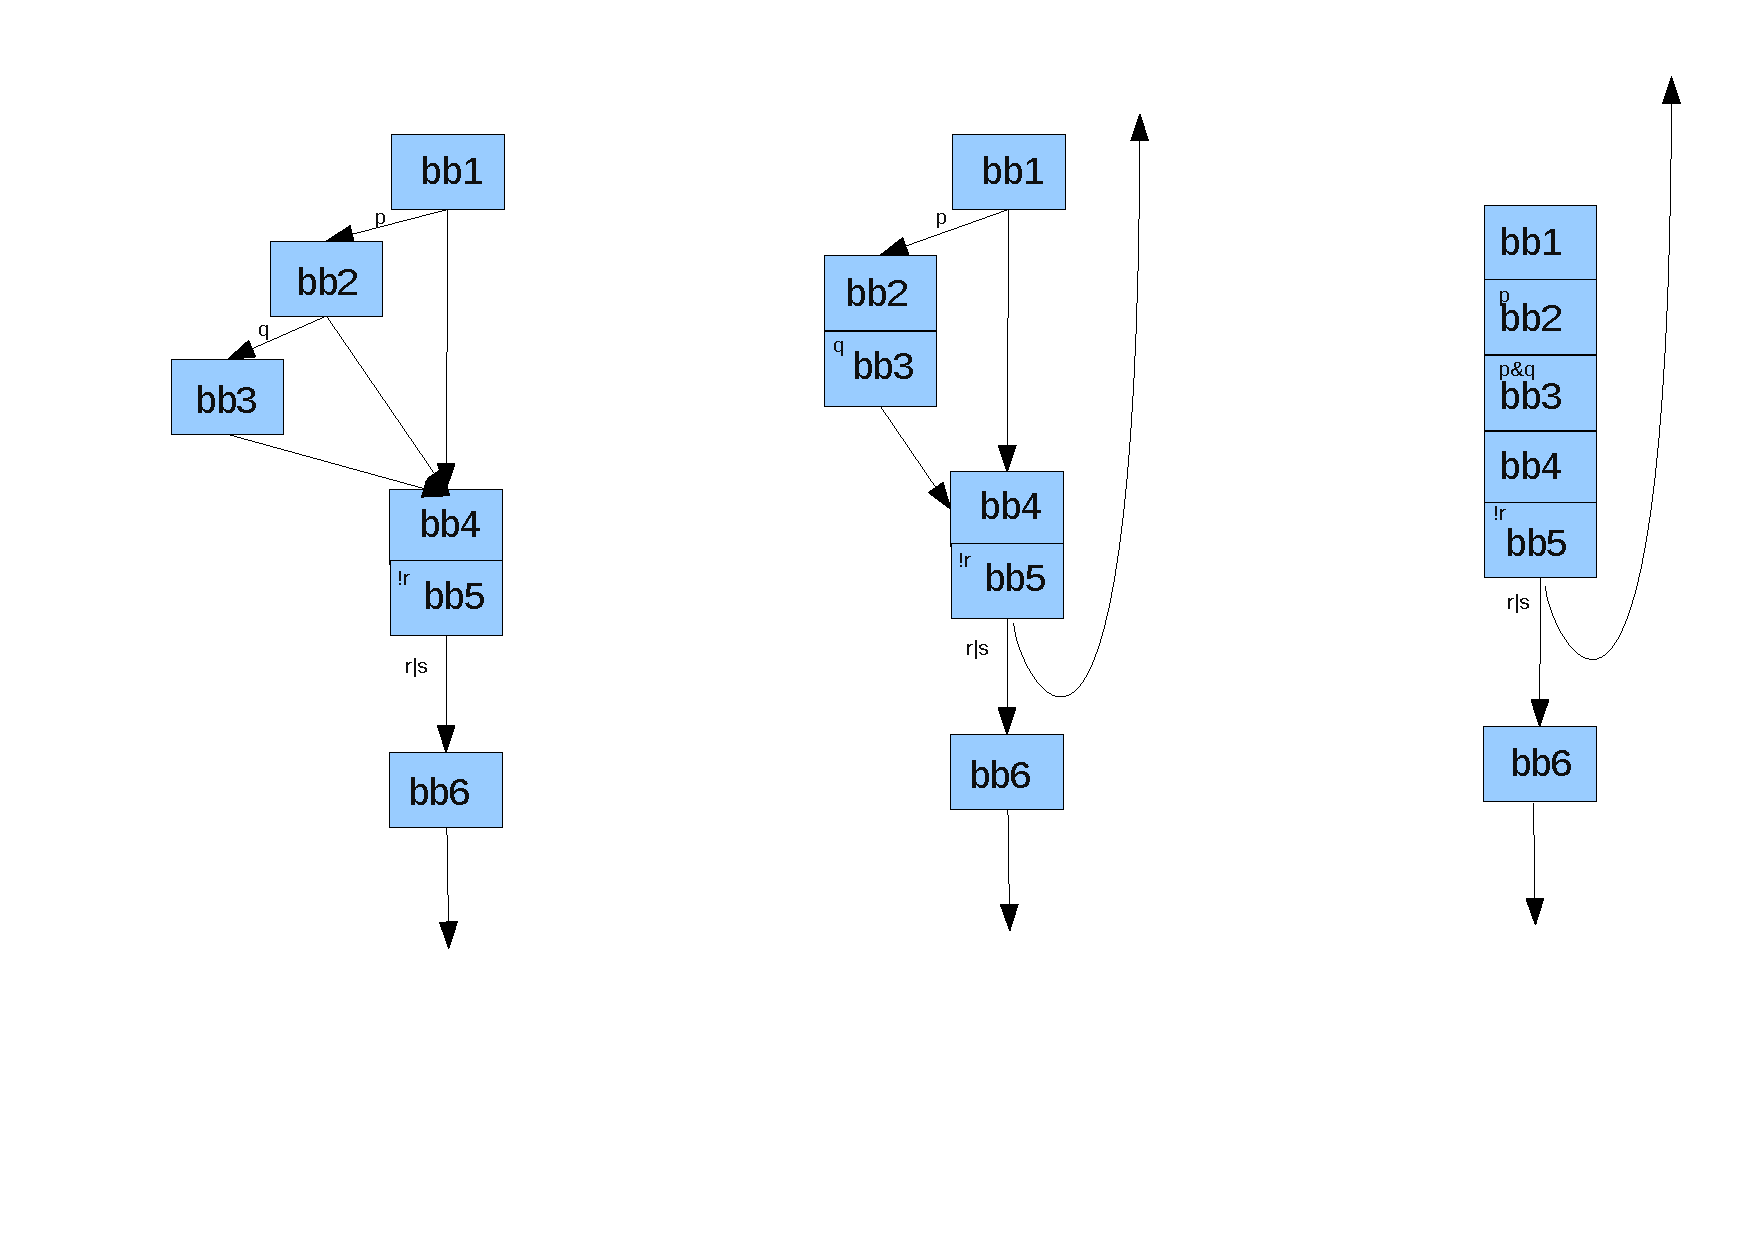
\includegraphics[scale=0.7]{hyper2}
    \label{fig:hyper2}}
  \subfloat[after SSA if-conversion] {
    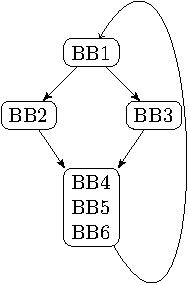
\includegraphics[scale=0.7]{hyper4}
    \label{fig:hyper4}}
  \subfloat[final flow] {
    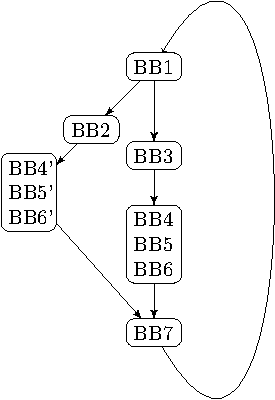
\includegraphics[scale=0.7]{hyper3}
    \label{fig:hyper3}}
\end{figure}

The fact that the if-conversion happens after tail-duplication. In the resulting code happens to be difficult to schedule efficiently, over committing resources. Hyperblock formation, if-conversion and speculation introduce a major phase ordering problem. A technique called ``Reverse If-Conversion'' \cite{August:1999:PRI:326224.325595} overcomes this problem, allowing use of an aggressive if-conversion framework and reconstructing the control flow at schedule time.

Consider in contrast how tail-duplication is performed in a lazy way, after the code have been if-converted. \ref{fig:hyper4} shows the same loop body where the second $if$ region has been SSA if-converted. The decision to if-convert the region formed by {BB1, BB2, BB3} is now local and can be taken conservatively. Only at this stage, if necessary, tail-duplication can be performed to remove the side entry coming from BB2. Duplicating a single predicated block is now a very simple operation.

\subsection{Profitability}

The decision to include a basic block into an hyperblock is one of the main difficult tradoff that a good if-conversion algorithm as to deal with. It should be aggressive enough to maximize the use of resources, but without overcomitting them, because of the risk of spilling registers or bad schedule if multiple instruction dependent of a scare resource. e.g a multiplier, a data bus a floating point unit. Conventional frameworks that separate the basic block selection from the if-conversion process have a hard time to find the good fit, and need sometime to do a reverse if-conversion \cite{August:1999:PRI:326224.325595}, when the choice appear at-posteriory to be too aggressive.

In contrast, the SSA iterative restructuring framework described earlier reduce the scope for the decision function to a very well localized. Furthermore, the predicate instructions or temporary register to hold the speculated instructions are already in the code that we are considering. Consequently, SSA iterative if-conversion construction is much more precise. The following factors are considered locally: 

- Semantic. The merge of different execution path should guarantee that the semantics of the program are preserved.
- If-conversion increases register pressure, for two reasons: live ranges are merged and register renaming imposes new constraints
- Schedule length: New data dependencies between a predicate definition and it's use, or between a speculated instruction and it's merge, can impede the schedule.

Since the execution cannot use dynamic branch prediction schemes to statically schedule the code, it is essential for the compiler to rely on accurate static branch prediction information \cite{Fisher:1992:PCB:143371.143493}. Using such information, the block selection process can decide whether the inclusion of one path into the other will be beneficial. 

The first consequence is that all registers are now live simultaneously, (live range), so the benefits of branch removal and better scheduling balanced with increased live range and register pressure : If-conversion must rely on an efficient decision model.

The basic idea for decision taking is that a region can be if-converted if the cost of the resulting if-converted basic block is smaller than the cost of each region taken separately weighted by the branch frequencies. The cost is a factor of 2 parameters: resource usage and schedule length.

We compare the pondered cost of the region before if-conversion. So the cost of a path is the schedule estimation of all the blocks in the path pondered by the probability of execution:
\begin{align}
Cost(path)=Freq(path)*\sum_{k=1}^n(Cost(bb_{k}))
\end{align}
The cost of the region starting at basic block $head$ before if-conversion is therefore the cost of all the basic blocks in the considered region, on each path.
\begin{align}
Cost(head)=Cost(bb_{head})+branch\:lat+Cost(taken\:path)+Cost(fall-though\:path)
\end{align}
One of the paths can be empty, in this case only the non empty path will be speculated and it has a zero cost. The Cost after if-conversion is estimated with:
\begin{align}
Cost(head)=Cost(bb_{head} o bb_{taken path} o bb_{fall-though path})
\end{align}

Where $o$ is the composition function that merges basic blocks together, removes associated branches and creates the predicate operations. The resulting $Cost$ applied to the new basic block represents the estimated schedule after if-conversion, that will be effective only if $Cost(head_{before\,ifc}) > Cost(head_{after\,ifc})$. 
 
The cost function uses the target's machine interface information for instruction latencies, resources usage and scheduling constraints to estimate the local scheduling. The local dependencies computed between instructions are used to compute the dependence height. The branch frequency is obtained either from static branch prediction heuristics, profile information or user inserted directives.
\begin{figure}
    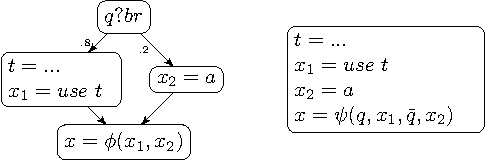
\includegraphics[scale=0.8]{ssa_freq}
\caption{example of profitable if-conversion}
\label{fig:ssa_freq}
\end{figure}

In example \ref{fig:ssa_freq} the dependence height of the fall-through path is 4 cycles. The dependence height of the taken path is 2 cycles. So the penetrated estimated cost of the region is 1+2.4+0.2+1=4.6 cycles. The estimated cost of the if-converted region is the schedule height estimation of the instructions without the branches. In this case, 4 cycles. Since the schedule height of the if-converted region is smaller than the profiled estimation, then it is profitable.
It should be noted that this heuristic does not take into account increased register pressure in the case of speculation, because the variables now interfere. Computing the inteference graph and simulating a register coalescing process would be extremely expensive at this stage. In the exampe above, a conservative approach would evaluate a register pressure of 4, without counting than $s$ and $t$ coalesce and that in reality the register budget would be 3. Note that this problem is general to every if-conversion algorithm, but might be more easy to deal with in the SSA framework because of the locality of the region.

\section{Conclusion} 
We presented in this chapter a novel if-conversion algorithm that takes advantage of the SSA properties to efficiently assign predicates and lay out the new control flow in an iterative, bottom up process. As opposed to the other top-down approach, this algorithm is very conservative, since the benefit of if-conversion is reevaluated at each nested transformation.
We show that we reunified region-formation and if-conversion into a single process, hyperblocks being created lazily, using well known techniques such as tail-duplication or branch coalescing only when the benefit is established.
Predication and speculation are often presented as two different alternatives for if-conversion. While it is true than they both require different hardware support, they should coexist in an efficient if-conversion process so every model of conditional execution is accepted. Thanks to conditional moves and $\psi$ transformations, they are now generated together in the same framework. The algorithm has been proved to be efficient in real world algorithms. For example, polynomial evaluation, for which specific ILP algorithm are designed can be fully if-converted in a straight-line of code \cite{JeKnMoRe11}, or we measured speedups up to 30\% on linux-scalar (spec benchs)  or embedded (eembc) application, without code size penalty.





